\documentclass{beamer}
\mode<presentation>
\usepackage{pgfpages}
\usetheme{iclpt}
\setbeamertemplate{navigation symbols}{}
\setbeamertemplate{headline}{
\begin{beamercolorbox}[leftskip=.2cm,rightskip=.2cm,topskip=.2cm,ht=1.1cm,dp=0.1cm,wd=\textwidth]{institute in head/foot}
  \includegraphics[height=1cm]{icl.pdf}
  \hfill
  
\includegraphics[height=1cm]{TalkPics/CMS-Color.eps}
\end{beamercolorbox}
}
\setbeamertemplate{footline}{
\begin{beamercolorbox}[ht=.55cm,dp=0.4cm,wd=\textwidth,leftskip=.3cm]{author in head/foot}%
  \begin{minipage}[c]{5cm}%
    \usebeamerfont{author in head/foot}
    \insertshortauthor 
    \insertshorttitle
    \end{minipage}\hfill%
  \insertframenumber{} / \inserttotalframenumber
  \hfill
  \begin{minipage}{6cm}
    \hfill
  \end{minipage}
\end{beamercolorbox}%
}


\title{Higgs Boson Searches at CMS}
\subtitle{What Have We Found So Far?}
\author{Patrick Dunne}
\date{}

\begin{document}

\section{Title}
\begin{frame}
  \titlepage
  \note[item]{Introduce yourself}
  \note[item]{Mention Invisible and Combinations}
\end{frame}


\section{Outline}
\begin{frame}{Outline}
  \begin{columns}
    \begin{column}{.5\textwidth}
      \begin{itemize}
      \item A Higgs-like boson was discovered in 2012 at the LHC.
      \item How did we decide we'd discovered something?
      \item How do we answer the question: ``Is it the Higgs?''
      \end{itemize}
    \end{column}
    \begin{column}{.5\textwidth}
      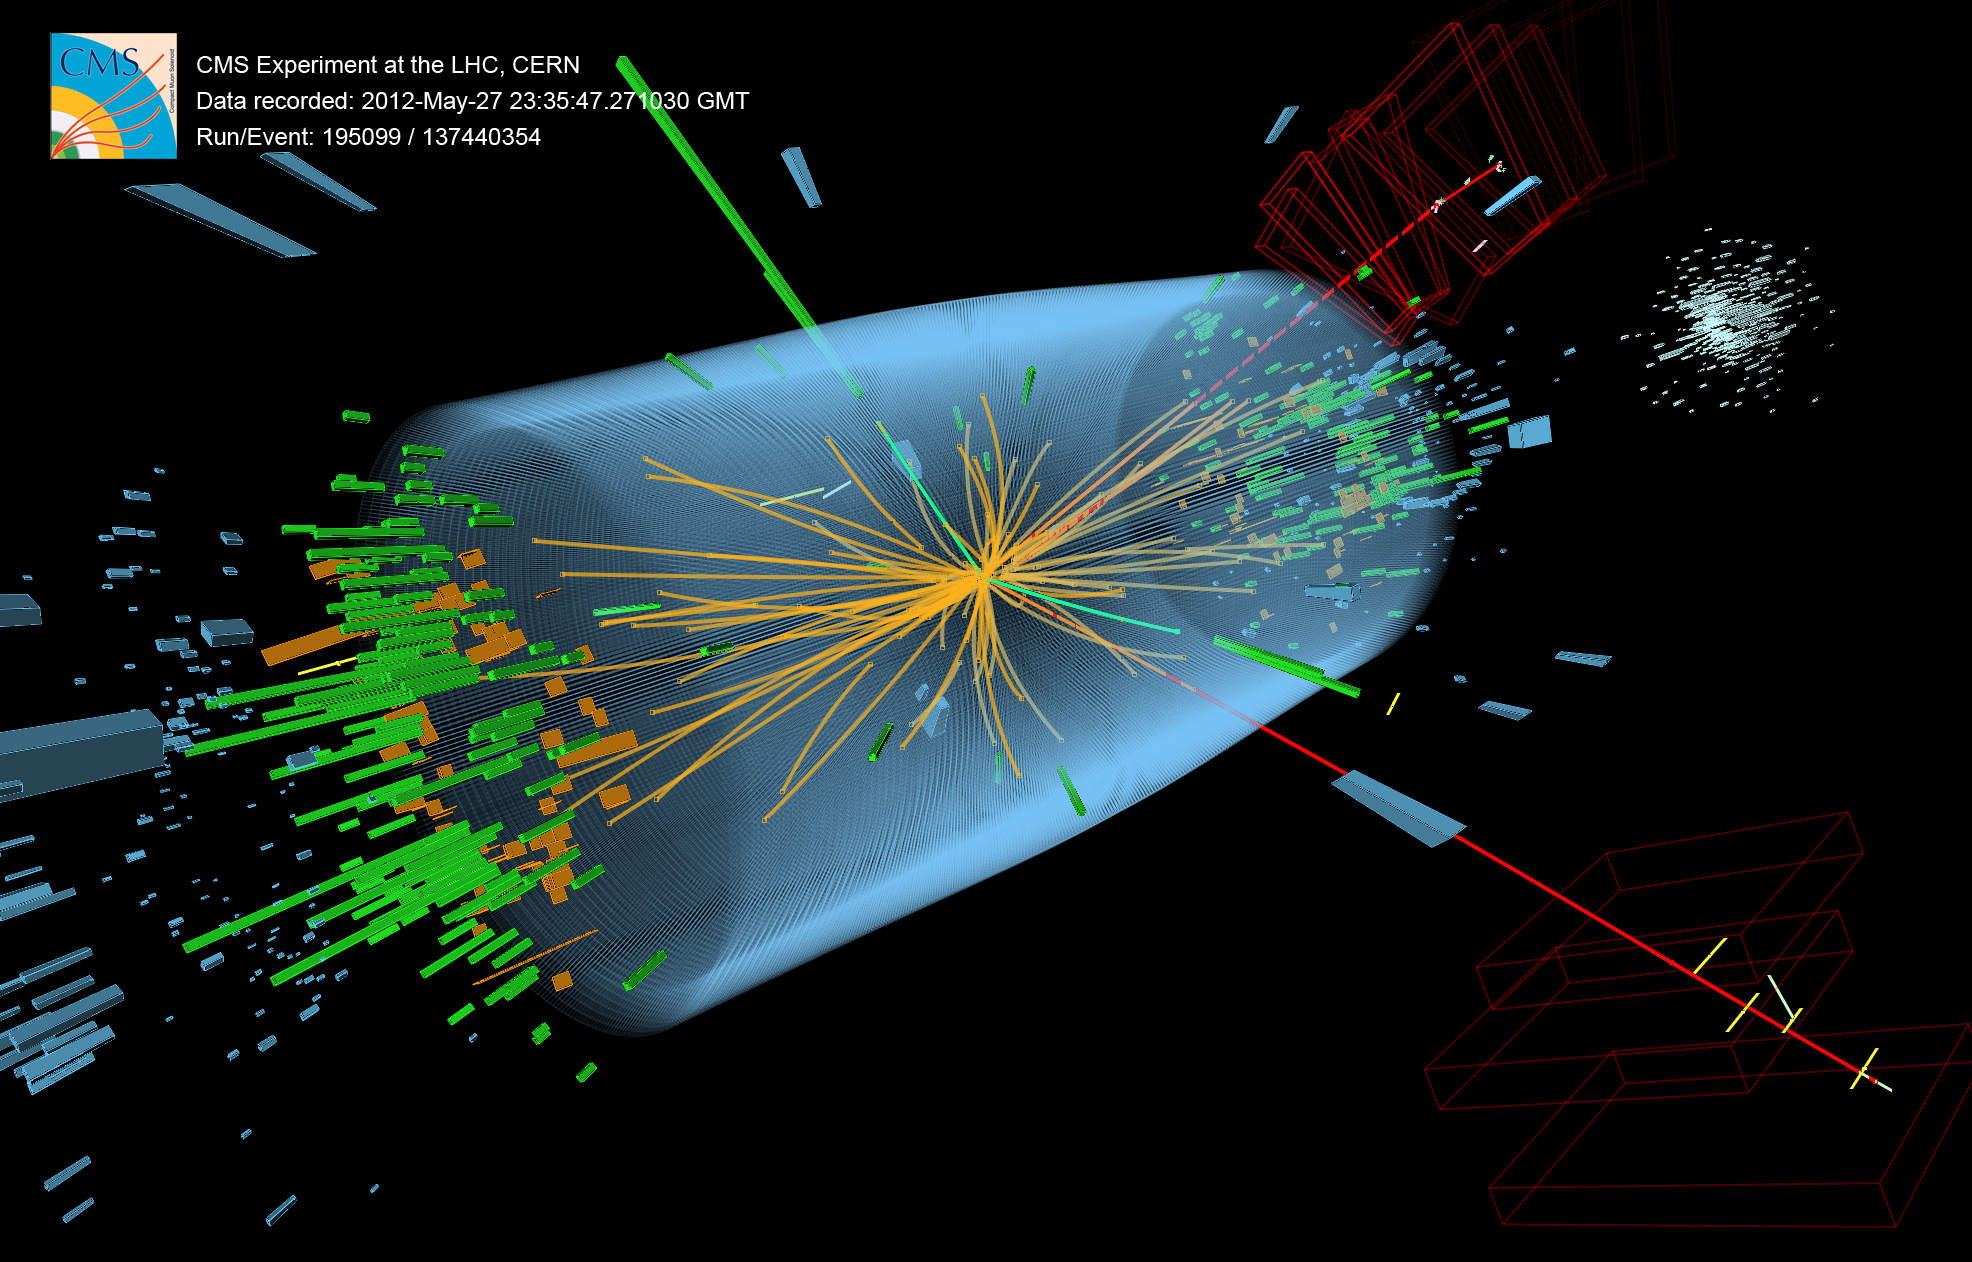
\includegraphics[width=\textwidth]{TalkPics/cmshtozzevent.png}
    \end{column}
  \end{columns}
\end{frame}


\section{The Standard Model and the Higgs Boson}
\begin{frame}{The Standard Model and the Higgs Boson}
  \begin{columns}
    \begin{column}{.6\textwidth}
      \begin{itemize}
      \item Higgs boson is a consequence of the Higgs mechanism which gives mass to the weak vector bosons
      \item Higgs mechanism also gives rise to the fermion masses
      \item Standard Model couplings are well predicted
      \end{itemize}
    \end{column}
    \begin{column}{.4\textwidth}
      %\begin{minipage}{\textwidth}
        %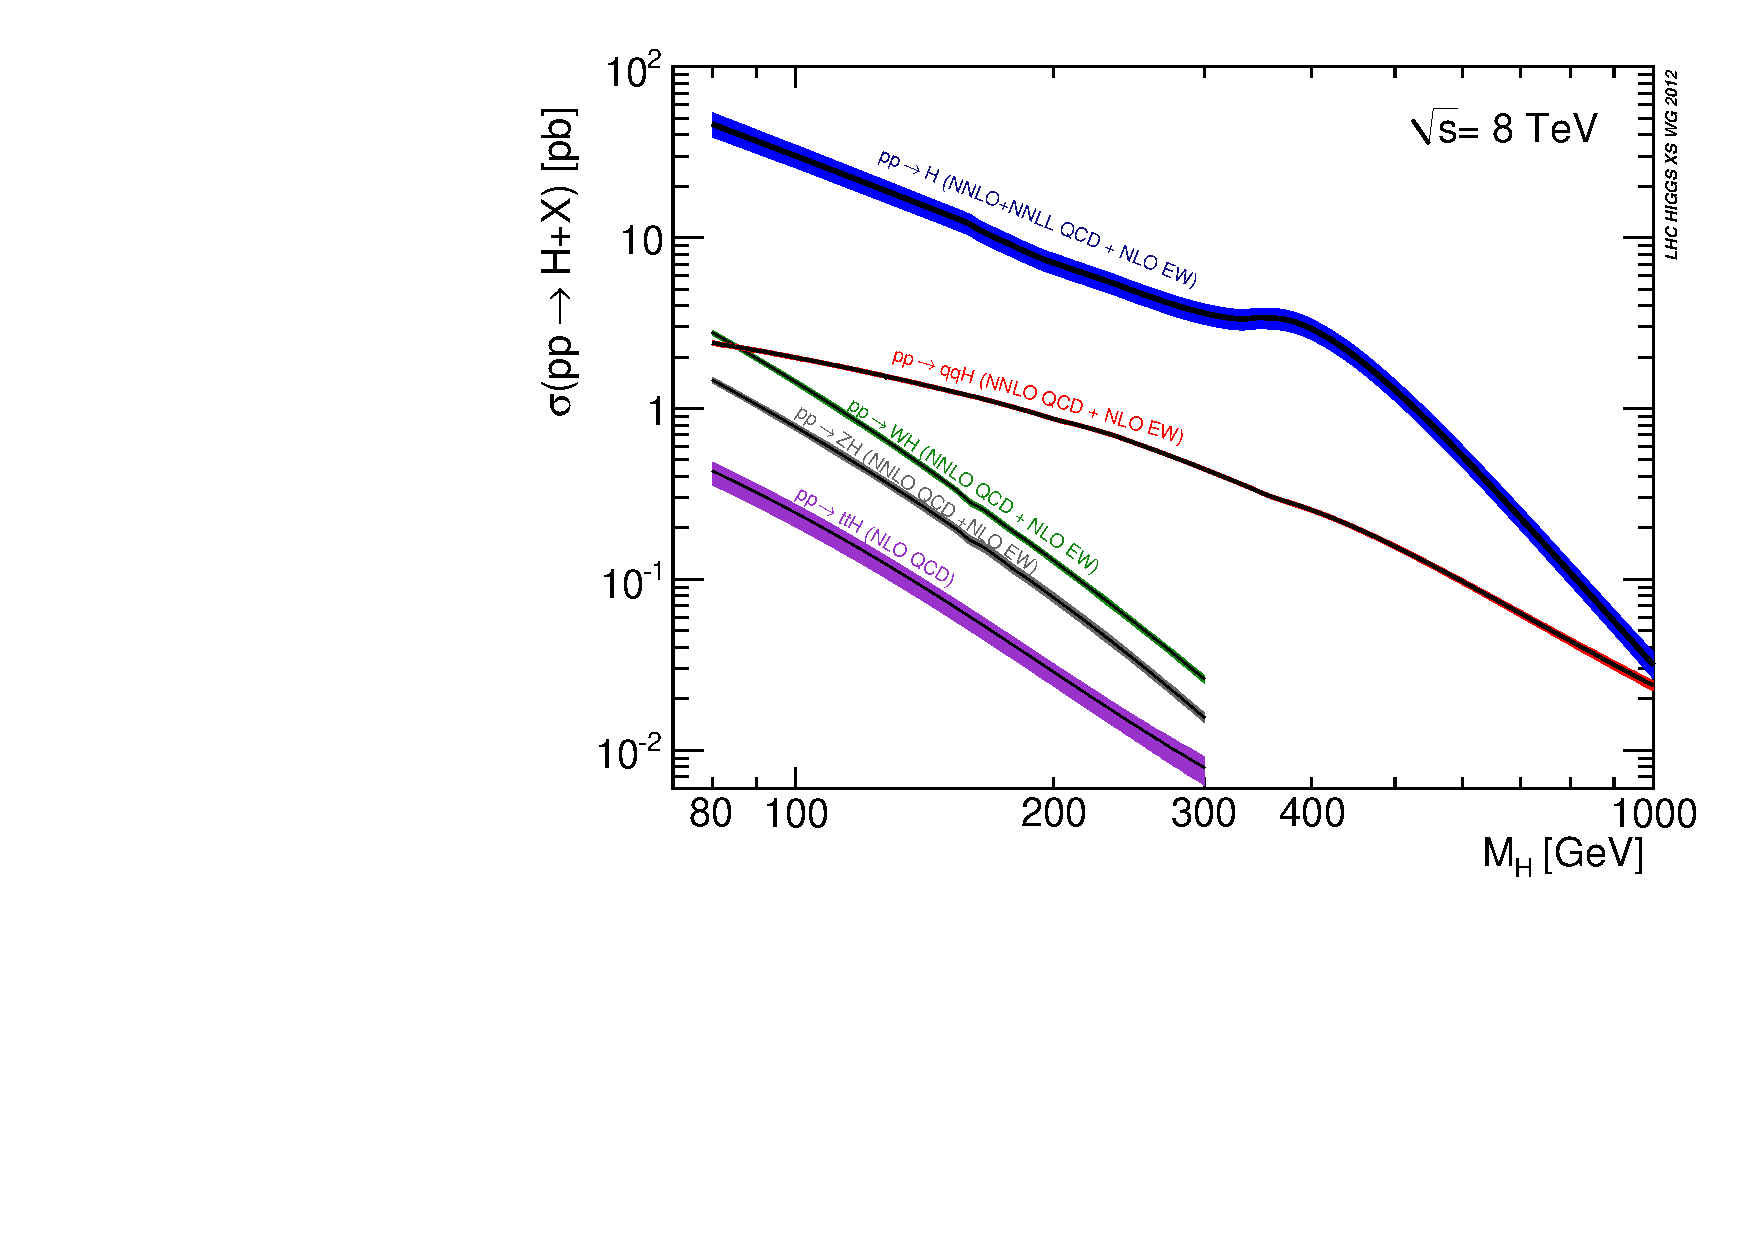
\includegraphics[height=.4\textheight]{Higgs_XS_8TeV_lx.pdf}
      %\end{minipage}
      \begin{minipage}{\textwidth}
        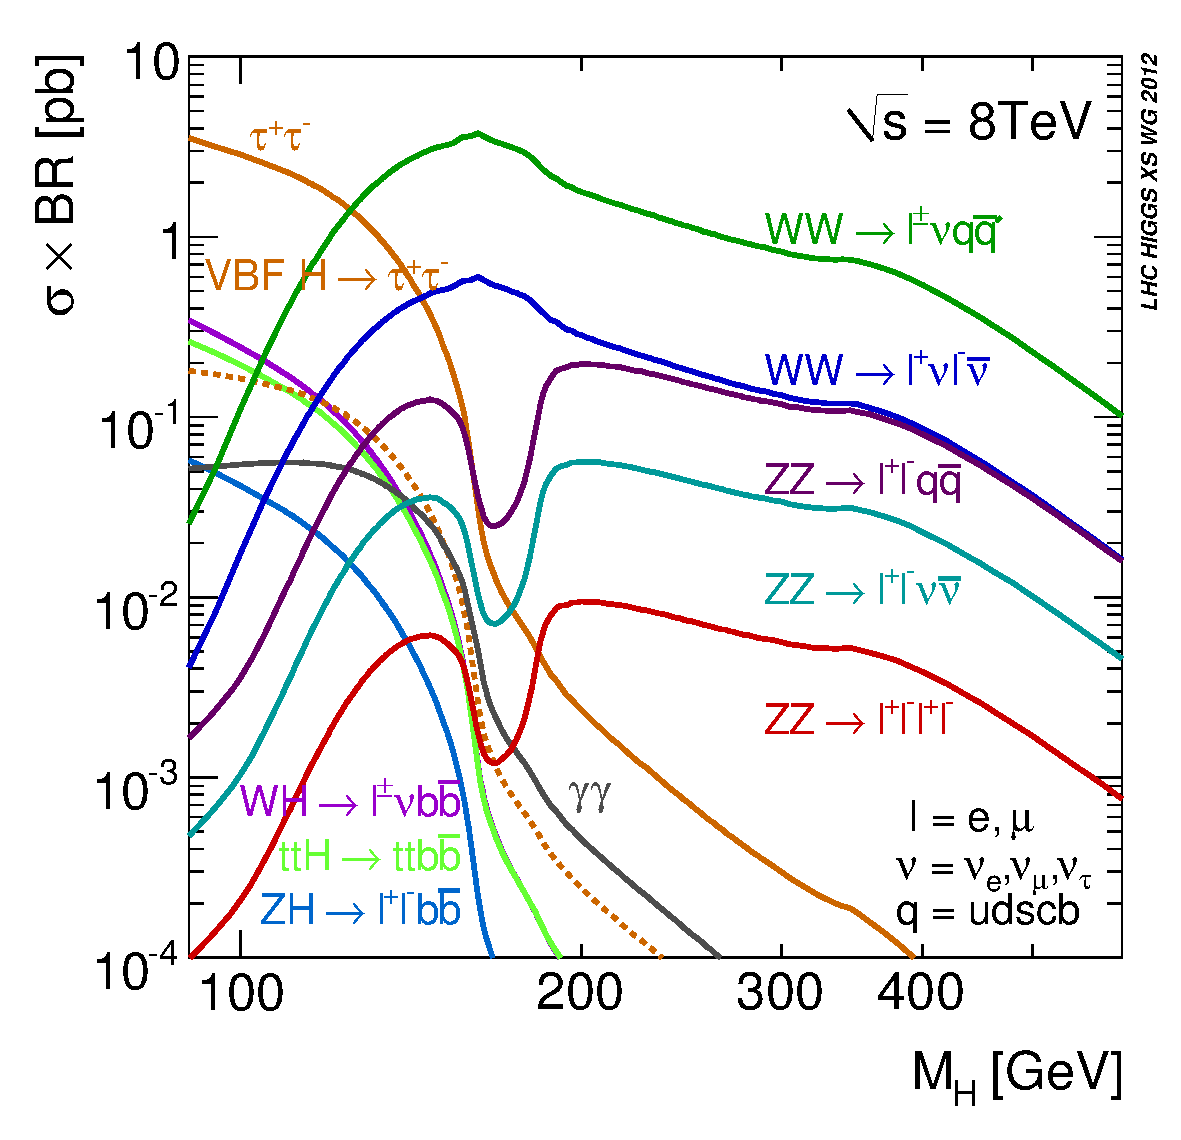
\includegraphics[width=\textwidth]{XSBR_8TeV_SM.pdf}
      \end{minipage}
    \end{column}
  \end{columns}
\end{frame}


\section{Combinations}
\begin{frame}{Combinations}
  \begin{itemize}
  \item To decide if we have found the Higgs boson we need to understand its properties
  \item This requires a combination of all the search channels
  \item The combination has three aims:
    \begin{itemize}
      \item<2-> Setting exclusion limits on the SM Higgs Boson
      \item<3-> Characterising excesses over the background
      \item<4-> Extracting signal model parameters from the data
    \end{itemize}
  \end{itemize}
\end{frame}


\subsection{Exclusion Limits}
\begin{frame}{Setting Exclusion Limits}
  \begin{itemize}
  \item The CL$_{s}$ statistic is used, which is the number of times more likely the signal hypothesis is than the background hypothesis.
  \item It is defined as:
    \begin{equation*}
    CL_{s} = \frac{P(q_{\mu}\geqslant q_{\mu}^{obs} | \mu \cdot s + b)}{P(q_{\mu}\geqslant q_{\mu}^{obs}|b)}
    \end{equation*}
  \item $\mu$ is a signal strength modifier
  \item q$_{\mu}$ is a profile likelihood ratio defined as:
    \begin{equation*}
      q_{\mu} = -2 \ln\frac{\mathcal{L}(obs|\mu \cdot s + b,\hat{\theta}_{\mu})}{\mathcal{L}(obs|\hat{\mu} \cdot s + b,\hat{\theta})}.
    \end{equation*}
  \end{itemize}
\end{frame}

\begin{frame}
  \frametitle<1>{2011 Exclusion}
  \frametitle<2>{Discovery Exclusion}
  \frametitle<3>{HCP Exclusion}
  \begin{figure}  
    \only<1>{\raisebox{-0.5\height}{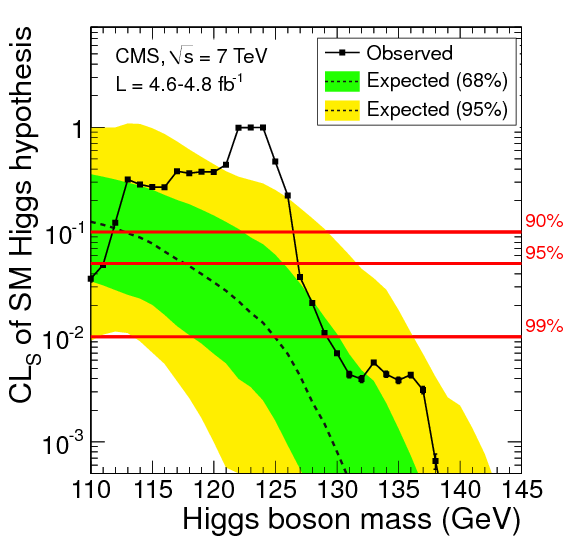
\includegraphics[width=0.49\textwidth]{TalkPics/exc2011lowmass.png}}}
    \only<1>{\raisebox{-0.5\height}{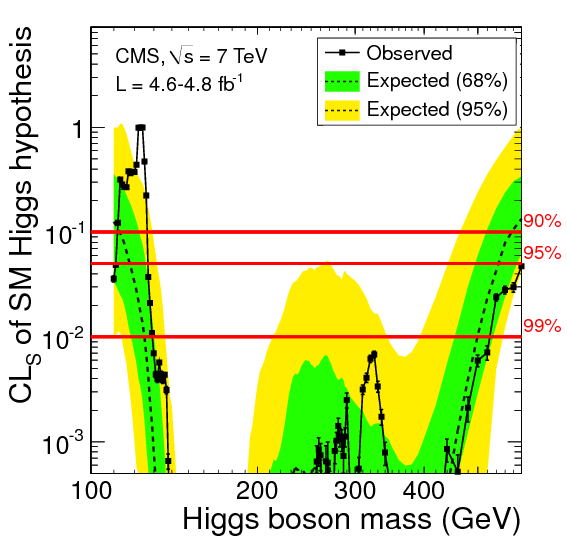
\includegraphics[width=0.49\textwidth]{TalkPics/exc2011fullrange.png}}}
    \only<2>{\raisebox{-0.5\height}{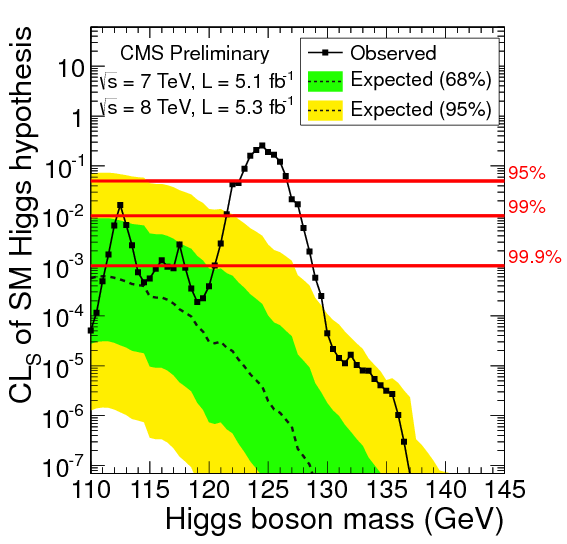
\includegraphics[width=0.49\textwidth]{TalkPics/excdisclowmass.png}}}
    \only<2>{\raisebox{-0.5\height}{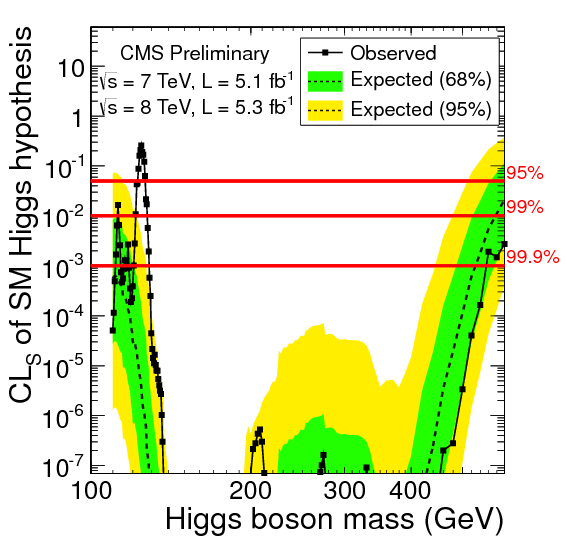
\includegraphics[width=0.49\textwidth]{TalkPics/excdiscfullrange.png}}}
    \only<3>{\raisebox{-0.5\height}{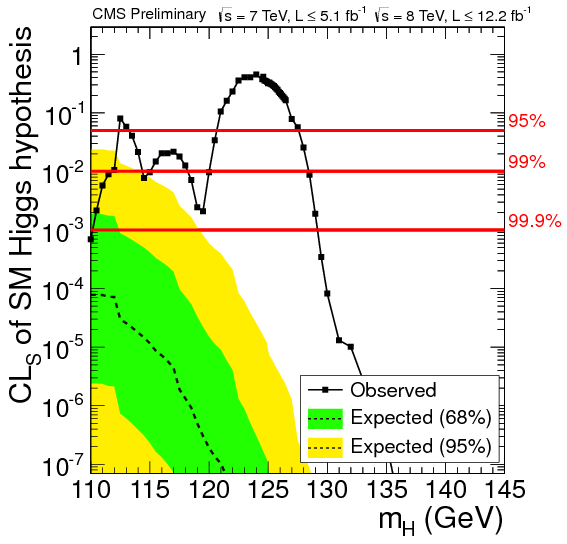
\includegraphics[width=0.49\textwidth]{TalkPics/exchcplowmass.png}}}
    \only<3>{\raisebox{-0.5\height}{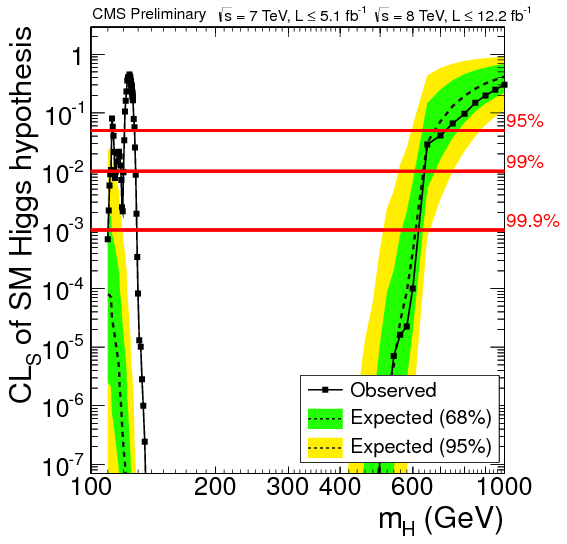
\includegraphics[width=0.49\textwidth]{TalkPics/exchcpfullrange.png}}}
  \end{figure}
\end{frame}


\subsection{Characterising Excesses}
\begin{frame}{Characterising Excesses}
  \begin{itemize}
  \item Higgs analyses use the  p value, defined as:
      \begin{equation*}
        p_{0} = P(q_{0} \leqslant q_{0}^{obs}|b),
      \end{equation*}
      \item q$_{0}$ is the profile likelihood from above with $\mu$ set to zero
      \item i.e. the p value is the probability of observing a background fluctuation as likely or less likely than that observed in the absence of signal.
      \item 1-p does not tell you P(signal)!
  \end{itemize}
\end{frame}

\begin{frame}
  \frametitle<1>{2011 Significance}
  \frametitle<2>{Discovery Significance}
  \frametitle<3>{HCP Significance}
  \begin{figure}  
    \only<1>{\raisebox{-0.5\height}{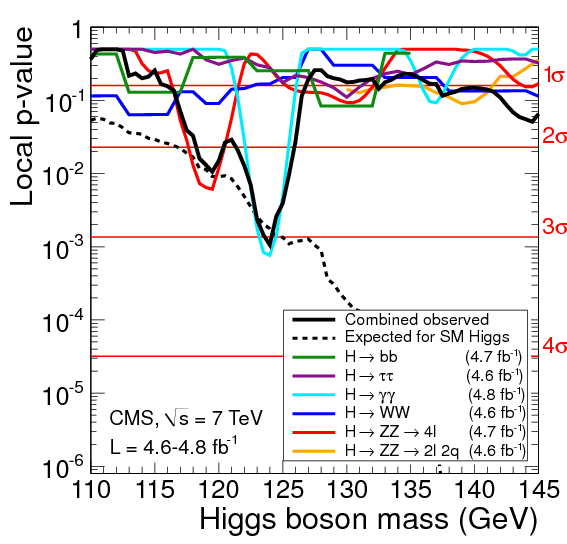
\includegraphics[width=0.49\textwidth]{TalkPics/sig2011.png}}}
    \only<2>{\raisebox{-0.5\height}{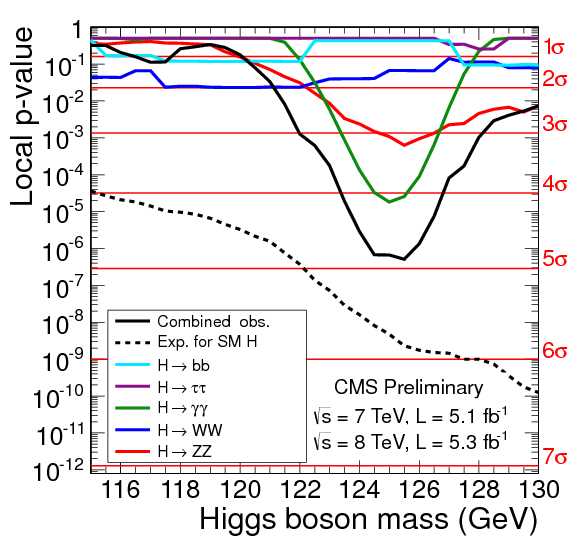
\includegraphics[width=0.49\textwidth]{TalkPics/sigdisc.png}}}
    \only<3>{\raisebox{-0.5\height}{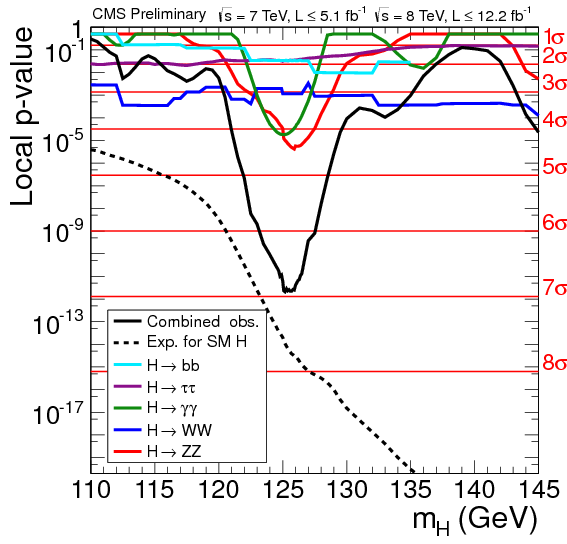
\includegraphics[width=0.49\textwidth]{TalkPics/sighcp.png}}}
  \end{figure}
\end{frame}


\subsection{Signal Parameter Determination}
\begin{frame}{Signal Parameter Determination}
  \begin{itemize}
  \item Most channels give their results in terms of $\sigma x BR$
  \item We want model parameters so another, slightly different, profile likelihood ratio is used
    \begin{equation*}
      q(a) = -2\ln\frac{\mathcal{L}(obs|s(a)+b,\hat{\theta}_{a})}{\mathcal{L}(obs|s(\hat{a})+b,\hat{\theta})}
    \end{equation*}
  \item a is the parameter of interest and hatted values are the values which maximise $\mathcal{L}$
  \item Basically a $\Delta$ log likelihood method so 1 $\sigma$ etc. contours can be plotted.
  \end{itemize}
\end{frame}

\begin{frame}
  \frametitle<1>{Mass}
  \frametitle<2>{Signal Strength}
  \frametitle<3>{Couplings}
  \begin{figure}  
    \only<1>{\raisebox{-0.5\height}{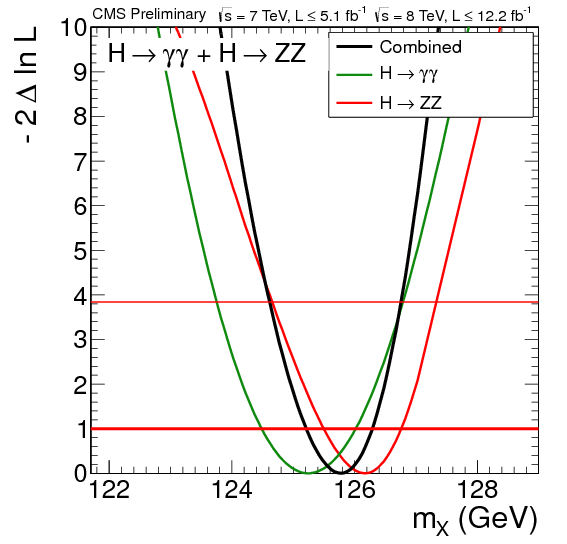
\includegraphics[width=0.49\textwidth]{TalkPics/parmass1d.png}}}
    \only<1>{\raisebox{-0.5\height}{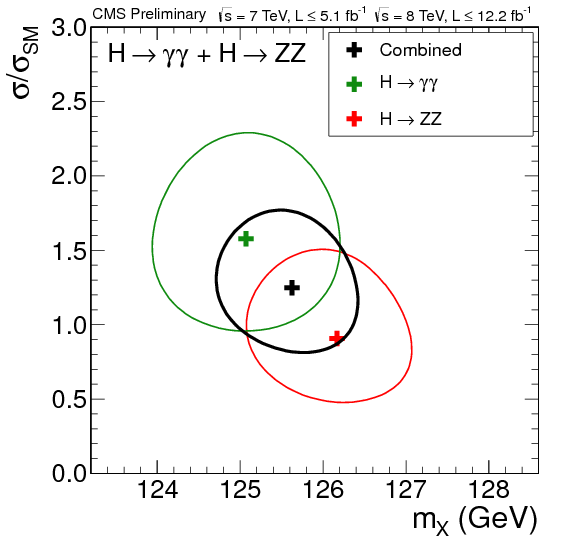
\includegraphics[width=0.49\textwidth]{TalkPics/parmass2d.png}}}
    \only<2>{\raisebox{-0.5\height}{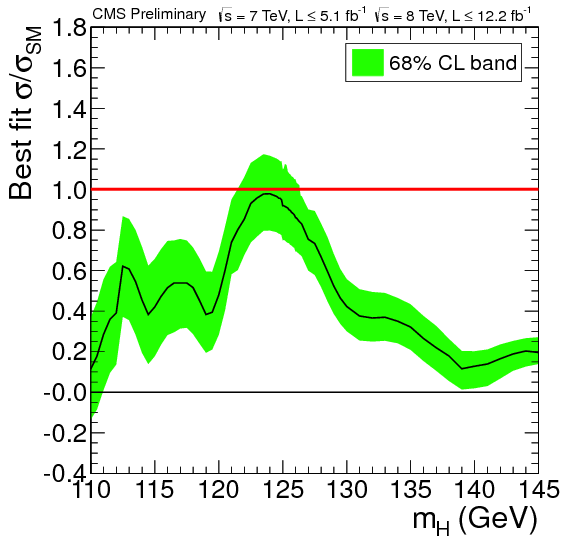
\includegraphics[width=0.49\textwidth]{TalkPics/parmu.png}}}
    \only<2>{\raisebox{-0.5\height}{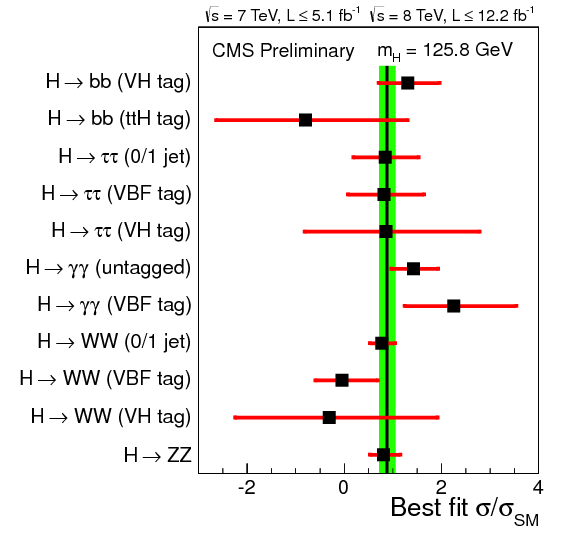
\includegraphics[width=0.49\textwidth]{TalkPics/parmuchans.png}}}
    \only<3>{\raisebox{-0.5\height}{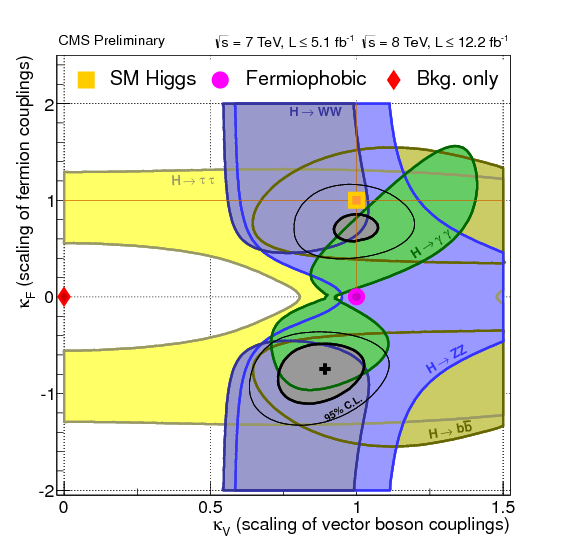
\includegraphics[height=.8\textheight]{TalkPics/parcoup.png}}}
  \end{figure}
  \end{frame}

\begin{frame}{What Next?}
  \begin{columns}
    \begin{column}{.5\textwidth}
      \begin{itemize}
      \item Finish analysing the 2012 dataset
      \item Analyse parked data
      \item Determine spin and parity
      \item Better coupling determination
        \end{itemize}
    \end{column}
    \begin{column}{.5\textwidth}
      \raisebox{-0.5\height}{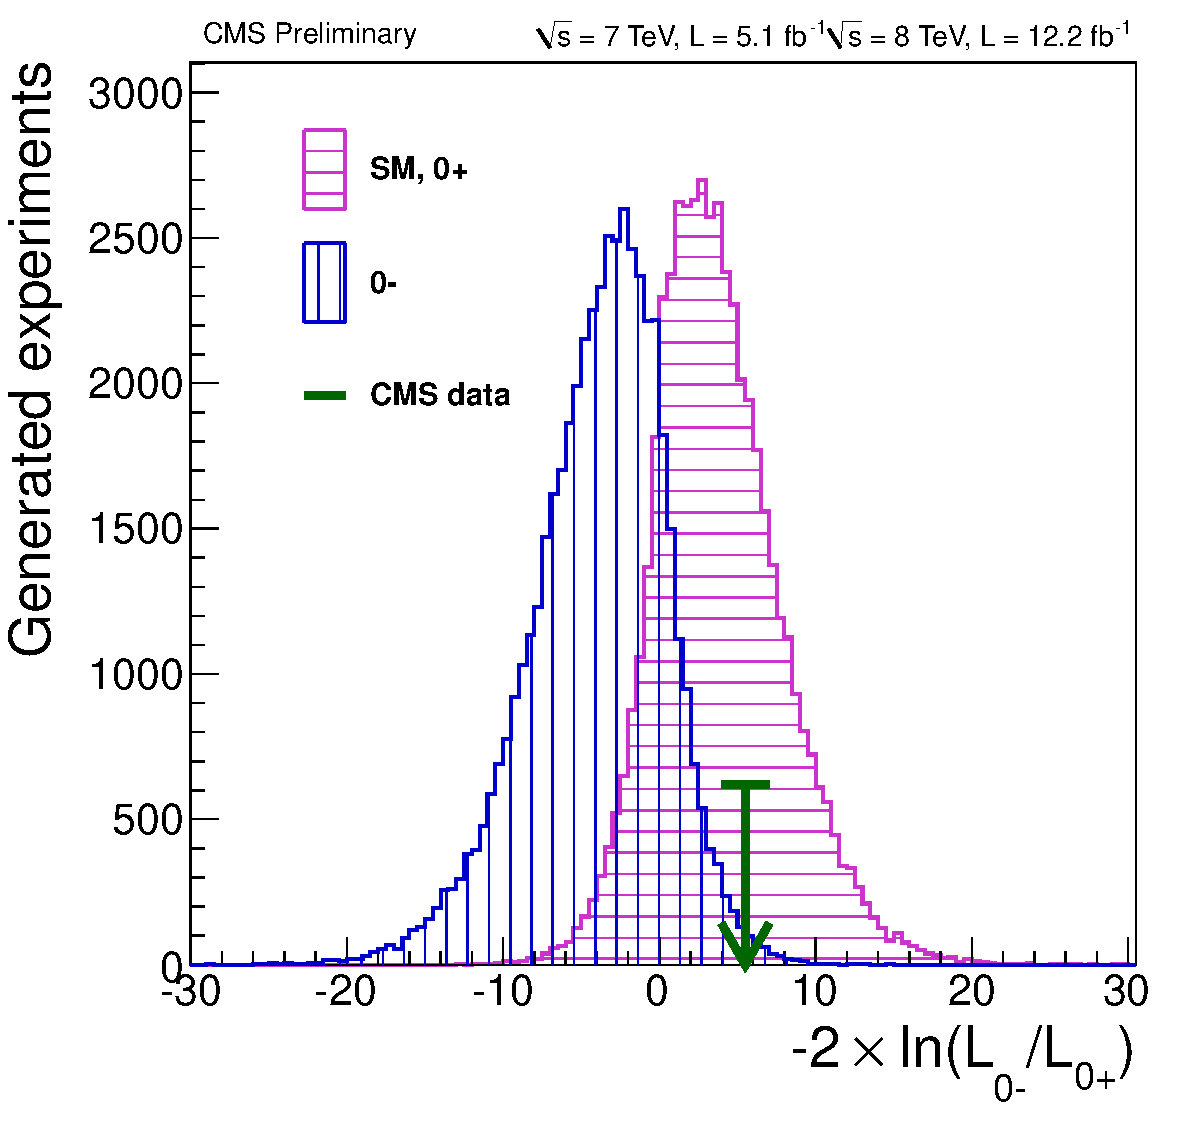
\includegraphics[height=.7\textheight]{TalkPics/spinparity.pdf}}
    \end{column}
  \end{columns}
\end{frame}


\end{document}
